
%\documentclass[11pts,a4paper,amsmath,amssymb,floatfix]{article}%{report}%{book}
\documentclass[12pts,a4paper,amsmath,amssymb,floatfix]{article}%{report}%{book}
\usepackage{graphicx,wrapfig,pdfpages}% Include figure files
%\usepackage{dcolumn,enumerate}% Align table columns on decimal point
\usepackage{enumerate,enumitem}% Align table columns on decimal point
\usepackage{bm,dpfloat}% bold math
\usepackage[pdftex,bookmarks,colorlinks=true,urlcolor=rltblue,citecolor=blue]{hyperref}
\usepackage{amsfonts,amsmath,amssymb,stmaryrd,indentfirst}
\usepackage{times,psfrag}
\usepackage{natbib}
\usepackage{color}
\usepackage{units}
\usepackage{rotating}
\usepackage{multirow}


\usepackage{pifont}
\usepackage{subfigure}
\usepackage{subeqnarray}
\usepackage{ifthen}

\usepackage{supertabular}
\usepackage{moreverb}
\usepackage{listings}
\usepackage{palatino}
%\usepackage{doi}
\usepackage{longtable}
\usepackage{float}
\usepackage{perpage}
\MakeSorted{figure}
%\usepackage{pdflscape}


%\usepackage{booktabs}
%\newcommand{\ra}[1]{\renewcommand{\arraystretch}{#1}}


\definecolor{rltblue}{rgb}{0,0,0.75}


%\usepackage{natbib}
\usepackage{fancyhdr} %%%%
\pagestyle{fancy}%%%%
% with this we ensure that the chapter and section
% headings are in lowercase
%%%%\renewcommand{\chaptermark}[1]{\markboth{#1}{}}
\renewcommand{\sectionmark}[1]{\markright{\thesection\ #1}}
\fancyhf{} %delete the current section for header and footer
\fancyhead[LE,RO]{\bfseries\thepage}
\fancyhead[LO]{\bfseries\rightmark}
\fancyhead[RE]{\bfseries\leftmark}
\renewcommand{\headrulewidth}{0.5pt}
% make space for the rule
\fancypagestyle{plain}{%
\fancyhead{} %get rid of the headers on plain pages
\renewcommand{\headrulewidth}{0pt} % and the line
}

\def\newblock{\hskip .11em plus .33em minus .07em}
\usepackage{color}

%\usepackage{makeidx}
%\makeindex

\setlength\textwidth      {16.cm}
\setlength\textheight     {22.6cm}
\setlength\oddsidemargin  {-0.3cm}
\setlength\evensidemargin {0.3cm}

\setlength\headheight{14.49998pt} 
\setlength\topmargin{0.0cm}
\setlength\headsep{1.cm}
\setlength\footskip{1.cm}
\setlength\parskip{0pt}
\setlength\parindent{0pt}


%%%
%%% Headers and Footers
\lhead[] {\text{\small{EX3029 -- Chemical Thermodynamics}}} 
\rhead[\text{\small{EOS and PVT behaviour assignment}}]{EOS and PVT behaviour assignment}
%\rfoot[] {{\text{\small{EOS + Mass Conservation using Matlab }}}}
%\chead[] {\text{\small{Session 2012/13}}} 
\lfoot[]{Dr Jeff Gomes}
\rfoot[\thepage]{\thepage}
\renewcommand{\headrulewidth}{0.8pt}


%%%
%%% space between lines
%%%
\renewcommand{\baselinestretch}{1.5}

\newenvironment{VarDescription}[1]%
  {\begin{list}{}{\renewcommand{\makelabel}[1]{\textbf{##1:}\hfil}%
    \settowidth{\labelwidth}{\textbf{#1:}}%
    \setlength{\leftmargin}{\labelwidth}\addtolength{\leftmargin}{\labelsep}}}%
  {\end{list}}

%%%%%%%%%%%%%%%%%%%%%%%%%%%%%%%%%%%%%%%%%%%
%%%%%%                              %%%%%%%
%%%%%%      NOTATION SECTION        %%%%%%%
%%%%%%                              %%%%%%%
%%%%%%%%%%%%%%%%%%%%%%%%%%%%%%%%%%%%%%%%%%%

% Text abbreviations.
\newcommand{\ie}{{\em{i.e., }}}
\newcommand{\eg}{{\em{e.g., }}}
\newcommand{\cf}{{\em{cf., }}}
\newcommand{\wrt}{with respect to}
\newcommand{\lhs}{left hand side}
\newcommand{\rhs}{right hand side}
% Commands definining mathematical notation.

% This is for quantities which are physically vectors.
\renewcommand{\vec}[1]{{\mbox{\boldmath$#1$}}}
% Physical rank 2 tensors
\newcommand{\tensor}[1]{\overline{\overline{#1}}}
% This is for vectors formed of the value of a quantity at each node.
\newcommand{\dvec}[1]{\underline{#1}}
% This is for matrices in the discrete system.
\newcommand{\mat}[1]{\mathrm{#1}}


\DeclareMathOperator{\sgn}{sgn}
\newtheorem{thm}{Theorem}[section]
\newtheorem{lemma}[thm]{Lemma}

%\newcommand\qed{\hfill\mbox{$\Box$}}
\newcommand{\re}{{\mathrm{I}\hspace{-0.2em}\mathrm{R}}}
\newcommand{\inner}[2]{\langle#1,#2\rangle}
\renewcommand\leq{\leqslant}
\renewcommand\geq{\geqslant}
\renewcommand\le{\leqslant}
\renewcommand\ge{\geqslant}
\renewcommand\epsilon{\varepsilon}
\newcommand\eps{\varepsilon}
\renewcommand\phi{\varphi}
\newcommand{\bmF}{\vec{F}}
\newcommand{\bmphi}{\vec{\phi}}
\newcommand{\bmn}{\vec{n}}
\newcommand{\bmns}{{\textrm{\scriptsize{\boldmath $n$}}}}
\newcommand{\bmi}{\vec{i}}
\newcommand{\bmj}{\vec{j}}
\newcommand{\bmk}{\vec{k}}
\newcommand{\bmx}{\vec{x}}
\newcommand{\bmu}{\vec{u}}
\newcommand{\bmv}{\vec{v}}
\newcommand{\bmr}{\vec{r}}
\newcommand{\bma}{\vec{a}}
\newcommand{\bmg}{\vec{g}}
\newcommand{\bmU}{\vec{U}}
\newcommand{\bmI}{\vec{I}}
\newcommand{\bmq}{\vec{q}}
\newcommand{\bmT}{\vec{T}}
\newcommand{\bmM}{\vec{M}}
\newcommand{\bmtau}{\vec{\tau}}
\newcommand{\bmOmega}{\vec{\Omega}}
\newcommand{\pp}{\partial}
\newcommand{\kaptens}{\tensor{\kappa}}
\newcommand{\tautens}{\tensor{\tau}}
\newcommand{\sigtens}{\tensor{\sigma}}
\newcommand{\etens}{\tensor{\dot\epsilon}}
\newcommand{\ktens}{\tensor{k}}
\newcommand{\half}{{\textstyle \frac{1}{2}}}
\newcommand{\tote}{E}
\newcommand{\inte}{e}
\newcommand{\strt}{\dot\epsilon}
\newcommand{\modu}{|\bmu|}
% Derivatives
\renewcommand{\d}{\mathrm{d}}
\newcommand{\D}{\mathrm{D}}
\newcommand{\ddx}[2][x]{\frac{\d#2}{\d#1}}
\newcommand{\ddxx}[2][x]{\frac{\d^2#2}{\d#1^2}}
\newcommand{\ddt}[2][t]{\frac{\d#2}{\d#1}}
\newcommand{\ddtt}[2][t]{\frac{\d^2#2}{\d#1^2}}
\newcommand{\ppx}[2][x]{\frac{\partial#2}{\partial#1}}
\newcommand{\ppxx}[2][x]{\frac{\partial^2#2}{\partial#1^2}}
\newcommand{\ppt}[2][t]{\frac{\partial#2}{\partial#1}}
\newcommand{\pptt}[2][t]{\frac{\partial^2#2}{\partial#1^2}}
\newcommand{\DDx}[2][x]{\frac{\D#2}{\D#1}}
\newcommand{\DDxx}[2][x]{\frac{\D^2#2}{\D#1^2}}
\newcommand{\DDt}[2][t]{\frac{\D#2}{\D#1}}
\newcommand{\DDtt}[2][t]{\frac{\D^2#2}{\D#1^2}}
% Norms
\newcommand{\Ltwo}{\ensuremath{L_2} }
% Basis functions
\newcommand{\Qone}{\ensuremath{Q_1} }
\newcommand{\Qtwo}{\ensuremath{Q_2} }
\newcommand{\Qthree}{\ensuremath{Q_3} }
\newcommand{\QN}{\ensuremath{Q_N} }
\newcommand{\Pzero}{\ensuremath{P_0} }
\newcommand{\Pone}{\ensuremath{P_1} }
\newcommand{\Ptwo}{\ensuremath{P_2} }
\newcommand{\Pthree}{\ensuremath{P_3} }
\newcommand{\PN}{\ensuremath{P_N} }
\newcommand{\Poo}{\ensuremath{P_1P_1} }
\newcommand{\PoDGPt}{\ensuremath{P_{-1}P_2} }

\newcommand{\metric}{\tensor{M}}
\newcommand{\configureflag}[1]{\texttt{#1}}

% Units
\newcommand{\m}[1][]{\unit[#1]{m}}
\newcommand{\km}[1][]{\unit[#1]{km}}
\newcommand{\s}[1][]{\unit[#1]{s}}
\newcommand{\invs}[1][]{\unit[#1]{s}\ensuremath{^{-1}}}
\newcommand{\ms}[1][]{\unit[#1]{m\ensuremath{\,}s\ensuremath{^{-1}}}}
\newcommand{\mss}[1][]{\unit[#1]{m\ensuremath{\,}s\ensuremath{^{-2}}}}
\newcommand{\K}[1][]{\unit[#1]{K}}
\newcommand{\PSU}[1][]{\unit[#1]{PSU}}
\newcommand{\Pa}[1][]{\unit[#1]{Pa}}
\newcommand{\kg}[1][]{\unit[#1]{kg}}
\newcommand{\rads}[1][]{\unit[#1]{rad\ensuremath{\,}s\ensuremath{^{-1}}}}
\newcommand{\kgmm}[1][]{\unit[#1]{kg\ensuremath{\,}m\ensuremath{^{-2}}}}
\newcommand{\kgmmm}[1][]{\unit[#1]{kg\ensuremath{\,}m\ensuremath{^{-3}}}}
\newcommand{\Nmm}[1][]{\unit[#1]{N\ensuremath{\,}m\ensuremath{^{-2}}}}

% Dimensionless numbers
\newcommand{\dimensionless}[1]{\mathrm{#1}}
\renewcommand{\Re}{\dimensionless{Re}}
\newcommand{\Ro}{\dimensionless{Ro}}
\newcommand{\Fr}{\dimensionless{Fr}}
\newcommand{\Bu}{\dimensionless{Bu}}
\newcommand{\Ri}{\dimensionless{Ri}}
\renewcommand{\Pr}{\dimensionless{Pr}}
\newcommand{\Pe}{\dimensionless{Pe}}
\newcommand{\Ek}{\dimensionless{Ek}}
\newcommand{\Gr}{\dimensionless{Gr}}
\newcommand{\Ra}{\dimensionless{Ra}}
\newcommand{\Sh}{\dimensionless{Sh}}
\newcommand{\Sc}{\dimensionless{Sc}}


% Journals
\newcommand{\IJHMT}{{\it International Journal of Heat and Mass Transfer}}
\newcommand{\NED}{{\it Nuclear Engineering and Design}}
\newcommand{\ICHMT}{{\it International Communications in Heat and Mass Transfer}}
\newcommand{\NET}{{\it Nuclear Engineering and Technology}}
\newcommand{\HT}{{\it Heat Transfer}}   
\newcommand{\IJHT}{{\it International Journal for Heat Transfer}}

\newcommand{\frc}{\displaystyle\frac}
\newcommand{\red}{\textcolor{red}}
\newcommand{\blue}{\textcolor{blue}}

\newlist{ExList}{enumerate}{1}
\setlist[ExList,1]{label={\bf Example 1.} {\bf \arabic*}}

\newlist{ProbList}{enumerate}{1}
\setlist[ProbList,1]{label={\bf Problem 1.} {\bf \arabic*}}

%%%%%%%%%%%%%%%%%%%%%%%%%%%%%%%%%%%%%%%%%%%
%%%%%%                              %%%%%%%
%%%%%% END OF THE NOTATION SECTION  %%%%%%%
%%%%%%                              %%%%%%%
%%%%%%%%%%%%%%%%%%%%%%%%%%%%%%%%%%%%%%%%%%%


% Cause numbering of subsubsections. 
%\setcounter{secnumdepth}{8}
%\setcounter{tocdepth}{8}

\setcounter{secnumdepth}{4}%
\setcounter{tocdepth}{4}%


\begin{document}

\begin{enumerate}[label=\bfseries Problem \arabic*:]
%
%%
%% Problem 1
%%
     \item\label{Prob1} Calculate the molar volume, $V\;\left(\text{in m}^{3}\text{.mol}^{-1}\right)$ and compressibility factor ($Z$) for gaseous ammonia at 450 K using the van der Waals (vdW) equation of state for the following conditions:
          \begin{enumerate}[label=\bfseries Task \arabic*]
              \item\label{c} {\bf[Hand calculation]} Pressure of 56 atm using the {\it generic cubic equation of state}; \hfill{\bf[12 Marks]}
              \item\label{d} Write a \underline{Matlab code} to obtain $V$ and $Z$ for reduced pressures $\left(P_{r}\right)$ of 0.1, 0.2, 0.5, 0.8, 1.0, 1.3, 1.5, 1.8 and 2.0. Plot $P_{r}\times Z$ and \underline{comment} the observed PVT behaviour of ammonia at this range of pressure based on EOS theory. \hfill{\bf[12 Marks]}
          \end{enumerate}
          Critical temperature and pressure of ammonia are 405.5 K and 111.3 atm, respectively.

%%
%% Problem 2
%%
     \item\label{Prob2} In order to investigate the PVT behaviour of gasses, 10$^{-3}$ m$^{3}$.mol$^{-1}$ of methanol is injected into a reactor cell and kept at constant temperature of 276.85$^{\circ}$C. Several properties of the gas were measured at reduced pressures $\left(P_{r}\right)$ ranging from 10$^{-5}$ to 1.  Similar measurements were obtained for benzene, toluene and carbon tetrachloride at the same conditions. Write a \underline{Matlab code} to calculate compressibility factor ($Z$) as a function of $P_{r}$ for both Soave-Redlich-Kwong (SRK-EOS) and Peng-Robinson (PR-EOS) cubic equations of state and solve the following tasks:
          \begin{enumerate}[label=\bfseries Task \arabic*]
              \item\label{a} Plot $P_{r}\times Z$ for all 4 gasses with both EOS; \hfill{\bf[20 Marks]} 
              \item\label{b} \underline{Using the data generated in} \ref{a} for PR-EOS, calculate pressures that will lead to $Z=0.750\pm0.001$ for all gasses. \hfill{\bf[10 Marks]} 
          \end{enumerate}
For your calculations, $10^{-5}\leq P_{r}\leq 1$ should be obtained with intervals of 10$^{-3}$, also you should use thermofluid properties from Table~\ref{Practical1:Table1}. 

\begin{table}[h]
\begin{center}
\begin{tabular}{||c | c c c c c ||} 
\hline\hline
                          & {\bf Molar Mass}           &  {\bf $\omega$}  & {\bf T$_{c}$}  & {\bf P$_{c}$} & {\bf Z$_{c}$}  \\
                          & $\left(\text{g.mol}^{-1}\right)$ &                  &   (K)         &   (bar)       &               \\ 
\hline
{\bf Benzene}             & 78.0                             &  0.212           &  563.0         &  49.2        &    0.271       \\  
{\bf Methanol}            & 32.0                             &  0.559           &  513.0         &  80.8        &    0.224       \\  
{\bf Toluene}             & 92.0                             &  0.266           &  592.0         &  41.3        &    0.284       \\  
{\bf Carbon tetrachloride}& 154.0                            &  0.194           &  556.0         &  45.6        &    0.272       \\  
\hline\hline
\end{tabular}
\caption{Thermofluid properties of fluids.}
\label{Practical1:Table1}
\end{center}
\end{table}

%%
%% Problem 3
%%
     \item An engineering consultancy company is contracted to design a separation process for a mixture of petroleum naphtha and fertilisers by-products. The mixture will be separated by a series of distillation and crystallisation processes. After the first distillation, lighter and heavier streams are stored in two pressure vessels:
         \begin{itemize}
            \item {\bf Vessel 1:} 45 mol-$\%$ of n-hexane, 30 mol-$\%$ of n-heptane and 25 mol-$\%$ of i-octane;
            \item {\bf Vessel 2:} 1.70 mol-$\%$ of n-hexane, 3.75 mol-$\%$ of n-heptane, 5.76 mol-$\%$ of i-octane, 27.45 mol-$\%$ of o-xylene, 37.71 mol-$\%$ of p-xylene and 23.63 mol-$\%$ of chlorobenzene.
         \end{itemize} 
         Vessels 1 and 2 are kept at 1.5 and 4.5 bar, respectively. In order to design the second set of distillations, a junior engineer needs to estimate bubble and dew temperatures (and vapour/liquid compositions) for the mixtures in both vessels. Thus:   
          \begin{enumerate}[label=\bfseries Task \arabic*]
              \item\label{e} {\bf[Hand-calculation]} Estimate the bubble and dew temperatures for Vessel 1. Also calculate the compositions at bubble and dew points;\hfill{\bf[20 Marks]}
              \item\label{f} Write a \underline{Matlab code} to calculate bubble and dew point temperatures and compositions at Vessel 2.\hfill{\bf[26 Marks]}
          \end{enumerate}
          Bubble and dew point are obtained through the following relations:
          \begin{displaymath}
             \sum\limits_{i=1}^{n} y_{i} = \sum\limits_{i=1}^{n} \frc{x_{i}P_{i}^{\text{sat}}}{P} = 1 \hspace{1cm}\text{ and } \hspace{1cm} \sum\limits_{i=1}^{n} x_{i} = \sum\limits_{i=1}^{n} \frc{y_{i}P}{P_{i}^{\text{sat}}} = 1,
          \end{displaymath}
          where $x_{i}$ and $y_{i}$ are molar fractions of component $i$ at liquid and vapour phases, respectively. $n$ and $P$ are the total number of components in the mixture and the system pressure. Finally, $P^{\text{sat}}$ is the vapour pressure that can be obtained from the Antoine equation,
          \begin{displaymath}
            \ln{P^{\text{sat}}} = A - \frc{B}{T+C}
          \end{displaymath}
          where $\left[P^{\text{sat}}\right]$ = kPa and $[T]$ = $^{\circ}$C, with coefficients given in Table~\ref{Practical1:Table2}.
           

\begin{table}[h]
\begin{center}
\begin{tabular}{||c | c c c ||} 
\hline\hline
                           & {\bf A}    &  {\bf B}    & {\bf C}    \\
\hline
{\bf n-hexane}             & 13.8193    & 2696.04     & 224.317    \\  
{\bf n-heptane}            & 13.8622    & 2910.26     & 216.432    \\  
{\bf i-octane}             & 13.6703    & 2896.31     & 220.767    \\  
{\bf o-xylene}             & 14.0415    & 3381.81     & 216.120    \\  
{\bf p-xylene}             & 14.0579    & 3331.45     & 214.627    \\  
{\bf chlorobenze}           & 13.8635    & 3174.78     & 211.700    \\  
\hline\hline
\end{tabular}
\caption{Constants for the Antoine equation for vapour pressure.}
\label{Practical1:Table2}
\end{center}
\end{table}




\end{enumerate}
\clearpage

{\bf Deliverables:}
\begin{itemize}
     \item Write a report containing a summary of your results (including figures, tables and equations) from the tasks and \underline{Matlab codes} used in your calculations. 
%
     \item {\bf Prepare the report and submit to the UG Office (with the appropriate plagiarism cover sheet) by Monday, October 31$^{st}$ 2016, \underline{noon} at the latest.}
%
     \item Feedback will be provided on November 21$^{st}$ 2016.
%
     \item Penalties for late or non-submission are as follows:
        \begin{enumerate}%[(a)]
            \item Up to one week late, 2 CGS points deducted;
            \item Up to two weeks late, 3 CGS point deducted;
            \item More than two weeks late no marks awarded.
        \end{enumerate}
        If late or non-submission is due to medical or other circumstances out with your control you must submit a medical certificate or other formal evidence to the UG Office as soon as is practicable but no later than the end of Revision Week.
%
     \begin{comment}
          If coursework is submitted late without prior arrangement, CGS marks will be deducted from the assessment mark as follows: 
             \begin{enumerate}
                \item up to one week late, 2 CGS points will be deducted;
                \item up to two weeks late, 3 CGS points will be deducted;
                \item up to three weeks late, 4 CGS points will be deducted, with a maximum achievable grade of CGS D3;
                \item up to four weeks late, 5 CGS points will be deducted, with a maximum achievable grade of CGS D3;
                \item more than four weeks late, NP will be recorded.
            \end{enumerate}
     \end{comment}
%
    \item Note that the submitted work is part of the continuous assessment which will contribute 20$\%$ to your EX3029 mark.
%
\end{itemize}



\clearpage

\begin{center}
  \Large{\bf Solutions}
\end{center}

Matlab codes used to solve this set of problems can be downloaded from the following link:
\begin{center}
    \href{https://www.dropbox.com/s/6uatv9ay9kelkq0/2016.zip?dl=0}{Matlab codes}
\end{center}

\begin{enumerate}[label=\bfseries Problem \arabic*:]
%  PROBLEM 1
   \item Solution:
      \begin{enumerate}[label=\bfseries Task \arabic*:]
          \item The generic form of cubic equations of state is defined as,
              \begin{displaymath}
                 Z = 1 + \beta - q\beta \frc{Z - \beta}{\left(Z+\epsilon\beta\right)\left(Z+\sigma\beta\right)}
              \end{displaymath}
              where 
              \begin{displaymath}
                 \beta = \Omega\frc{P_{r}}{T_{r}}\;\;\text{and}\;\; q = \frc{\Psi\alpha}{\Omega T_{r}}
              \end{displaymath}
              For vdW-EOS:
              \begin{displaymath}
                  \Omega = \frc{1}{8},\; \Psi=\frc{27}{64},\; \alpha=1,\; \epsilon = 0\;\text{ and }\; \sigma=0
              \end{displaymath}
              Reduced pressure and temperature are \blue{(\underline{2 marks})}:
              \begin{displaymath}
                  P_{r} = \frc{P}{P_{c}} = 0.5031,\;\;\text{ and }\;\; T_{r} = \frc{T}{T_{r}} 1.1097
              \end{displaymath}
              $\beta$ and $q$ are \blue{(\underline{2 marks})}:
              \begin{displaymath}
                 \beta = 5.6671\times 10^{-2}\;\;\text{ and }\;\; q = 3.0414
              \end{displaymath}
              We can simplify the generic form of cubic EOS as,
              \begin{displaymath}
                  Z =  1 + \beta - q\beta\frc{Z-\beta}{Z^{2}}
              \end{displaymath}
              And solving it (calculator), we can obtain Z = 0.8718 \blue{(\underline{6 marks})}. Molar volume can be obtained through \blue{(\underline{2 marks})}
              \begin{displaymath}
                  V = \frc{Z R T}{P} = 5.7482\times 10^{-4}\;\text{m}^{3}.\tex{mol}^{-1}
              \end{displaymath}

          \item Use the Matlab code in the {\it Problem 1} directory to plot $P_{r}\times Z$ \blue{(\underline{8 marks})}.  Initially ammonia was at vapour phase with temperature of 450 K (therefore above the critical temperature) and pressure of 11.13 atm (at $P_{r}$=0.1, therefore below critical pressure). At such relatively low pressure, gaseous ammonia behaves very similarly to an ideal gas (Z = 0.9766). However, as pressure (and reduced pressure) is increased, $Z$ is sharply reduced as it approaches the critical region $\left(P_{r}=1\right)$. After this point $\left(P_{r}>1\text{ and }T_{r}>1\right)$, ammonia is at supercritical state and the vdW (in fact, any cubic EOS) is no longer adequate to represent the PVT behaviour of the fluid \blue{(\underline{4 marks})}.
            \begin{figure}[h]
               \begin{center}
                   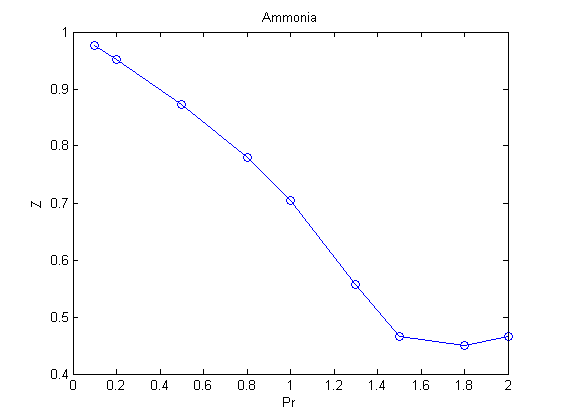
\includegraphics[width=12.cm,height=8.cm,clip]{./Figs/NH3.png}
               \end{center}
               \caption{Problem 1, Task 2. }
               \label{Prob2_Task2}
            \end{figure}

      \end{enumerate} 

\clearpage

% PROBLEM 2
   \item Use the Matlab code in the {\it Problem 2} directory:
      \begin{enumerate}[label=\bfseries Task \arabic*:]
        \item Each plot is worth \blue{\underline{5 marks}}. See Matlab code for the solution.
          \begin{figure}[h]
             \vbox{
                   \hbox{ 
                          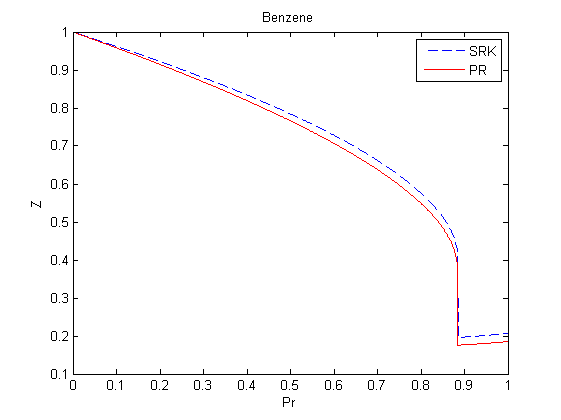
\includegraphics[width=8.cm,height=6.cm,clip]{./Figs/Benzene.png}
                          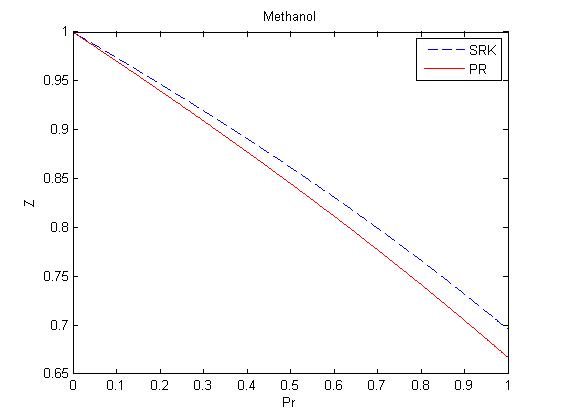
\includegraphics[width=8.cm,height=6.cm,clip]{./Figs/Methanol.png}
                         }
                   \hbox{ 
                          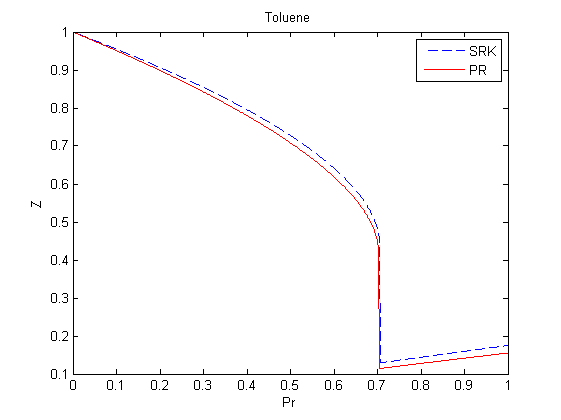
\includegraphics[width=8.cm,height=6.cm,clip]{./Figs/Toluene.png}
                          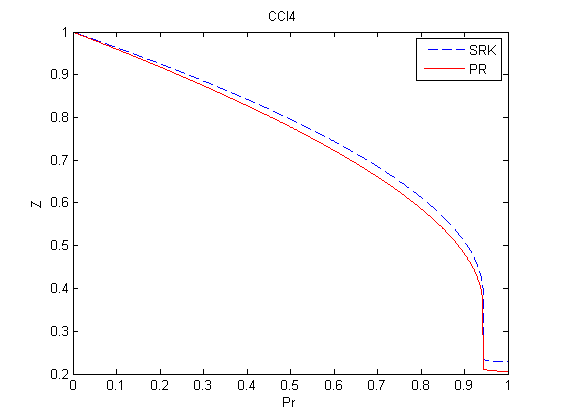
\includegraphics[width=8.cm,height=6.cm,clip]{./Figs/CCl4.png}
                        }
                  } 
             \caption{Problem 1, Task 1. }
             \label{Prob1_Task1}
          \end{figure}
%
        \item Using the Matlab code, one can obtain pressures in the following range (depending on number of points or the method used) (\blue{\underline{2.5 marks}} each): 
          \begin{itemize}
             \item Methanol:  62.62 - 63.02 bar
             \item Benzene:   25.98 - 26.08 bar
             \item Toluene:   18.30 - 18.38 bar
             \item CCl$_{4}$:  25.13 - 25.26 bar
          \end{itemize}
      \end{enumerate} 
\clearpage

% PROBLEM 3
   \item For Task 2, use the Matlab code in the {\it Problem 3} directory.
      \begin{enumerate}[label=\bfseries Task \arabic*:]
%
         \item Hand calculation:
            \begin{enumerate}
               \item Bubble point \blue{(\underline{2 marks})}:
                    \begin{eqnarray}
                        \sum\limits_{i=1}^{n} y_{i} &=& \sum\limits_{i=1}^{n} \frc{x_{i}P_{i}^{\text{sat}}}{P} = 1 \nonumber \\
                        &=& \frc{x_{C6}P_{C6}^{\text{sat}}}{P} + \frc{x_{C7}P_{C7}^{\text{sat}}}{P} + \frc{x_{C8}P_{C8}^{\text{sat}}}{P} = 1 \nonumber \\
                                                 &=& x_{C6}P_{C6} + x_{C7}P_{C7} + x_{C8}P_{C8} = P, \nonumber 
                    \end{eqnarray}
                    with the Antoine relation,
                      \begin{displaymath}
                         \ln{P^{\text{sat}}} = A - \frc{B}{T+C},
                      \end{displaymath}
                     with $P$ 150 kPa. Solving this non-linear equation (using a calculator) leads to the bubble point temperature $\Longrightarrow$ $T_{\text{bubble}}$ = 95.68$^{\circ}$C (\blue{\underline{5 marks}}).  Vapour phase composition is obtained from:
                      \begin{displaymath}
                         y_{i} = \frc{x_{i}P_{i}^{\text{sat}}}{P}.
                      \end{displaymath}
                      Leading to y = [ 0.6603, 0.1870, 0.1527 ] (\blue{\underline{3 marks}}).
%
               \item Dew point \blue{(\underline{2 marks})}:
                    \begin{eqnarray}
                        \sum\limits_{i=1}^{n} x_{i} &=& \sum\limits_{i=1}^{n} \frc{y_{i}P}{P_{i}^{\text{sat}}} = 1 \nonumber \\
                                                 &=& \frc{y_{C6}P}{P_{C6}^{\text{sat}}} + \frc{y_{C7}P}{P_{C7}^{\text{sat}}} + \frc{y_{C8}P}{P_{C8}^{\text{sat}}} = 1 \nonumber 
                    \end{eqnarray}
                    Solving this non-linear equation (using a calculator) leads to the dew point temperature $\Longrightarrow$ $T_{\text{dew}}$ = 102.10$^{\circ}$C (\blue{\underline{5 marks}}).  Liquid phase composition is obtained from:
                      \begin{displaymath}
                         x_{i} = \frc{y_{i}P}{P_{i}^{\text{sat}}}.
                      \end{displaymath}
                      Leading to x = [ 0.2599, 0.3989, 0.3412 ] (\blue{\underline{3 marks}}).    
            \end{enumerate}
%
          \item From Matlab code:
            \begin{enumerate}
               \item Bubble temperature: 195.95$^{\circ}$C (\blue{\underline{7 marks}}) with vapour composition of (\blue{\underline{6 mark}})
                   \begin{center}
                      y = [ 0.0620, 0.0752, 0.1061, 0.2086, 0.3196, 0.2285]
                   \end{center}
                   for n-C$_{6}$, n-C$_{7}$, i-C$_{8}$, o-xylene, p-xylene and chlorobenzene.
               \item Dew temperature: 201.14$^{\circ}$C (\blue{\underline{7 marks}}) with liquid composition of (\blue{\underline{6 mark}})
                   \begin{center}
                      x = [ 0.0043, 0.0171, 0.0287, 0.3262, 0.4021, 0.2216].
                   \end{center}
            \end{enumerate}
%
      \end{enumerate} 
%
\end{enumerate}


\end{document}
